% !TEX root = ../main.tex
% Graphic for TeX using PGF
% Title: /Applications/Dia.app/Diagramme1.dia
% Creator: Dia v0.97.2
% CreationDate: Thu Feb 27 13:32:45 2020
% For: marchann
% \usepackage{tikz}
% The following commands are not supported in PSTricks at present
% We define them conditionally, so when they are implemented,
% this pgf file will use them.
\ifx\du\undefined
  \newlength{\du}
\fi
\setlength{\du}{13\unitlength}
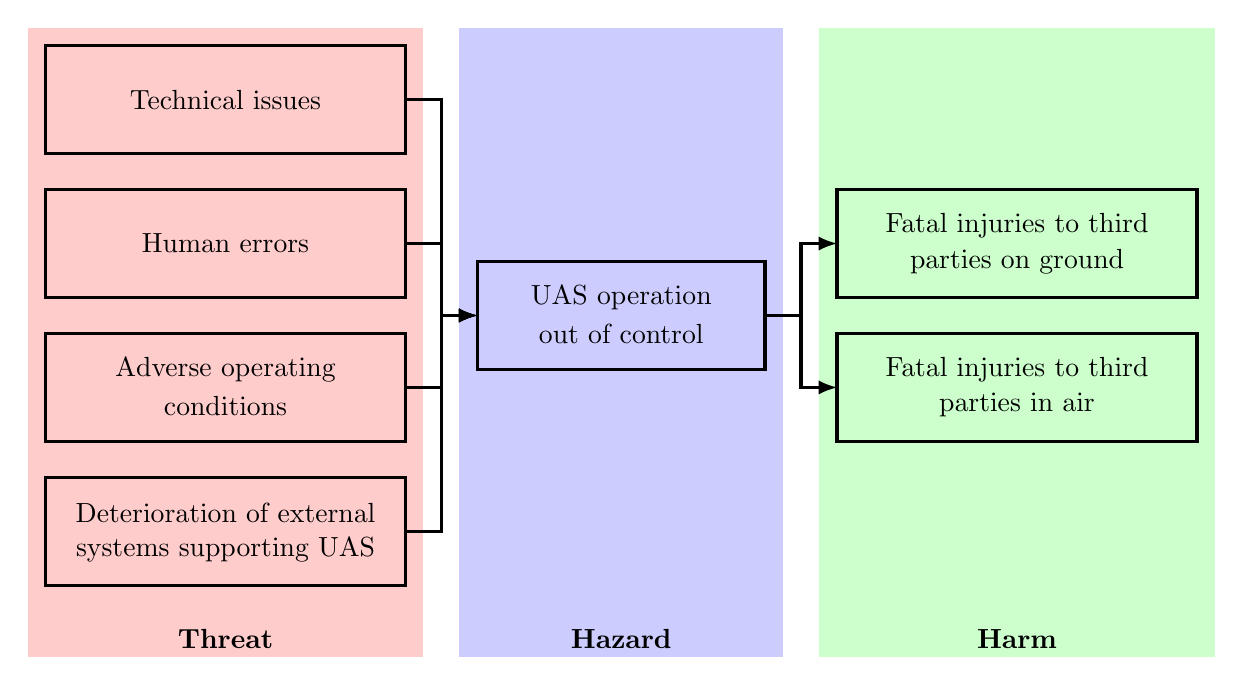
\begin{tikzpicture}
\pgftransformxscale{1.000000}
\pgftransformyscale{-1.000000}
\pgfsetlinewidth{0.100000\du}

%%%%%%%%%%%%%%%% Boites %%%%%%%%%%%%%%
\fill[color=red!20] (-.5\du,-.5\du)--(-.5\du,17\du)--(10.5\du,17\du)--(10.5\du,-.5\du)--cycle;
\node at (5\du,16.5\du){\bf Threat};

\pgfsetstrokecolor{black}
\draw (0\du,0\du)--(0\du,3\du)--(10\du,3\du)--(10\du,0\du)--cycle;
\node at (5\du,1.5\du){Technical issues};
\draw (0\du,4\du)--(0\du,7\du)--(10\du,7\du)--(10\du,4\du)--cycle;
\node at (5\du,5.5\du){Human errors};
\draw (0\du,8\du)--(0\du,11\du)--(10\du,11\du)--(10\du,8\du)--cycle;
\node at (5\du,9\du){Adverse operating};
\node at (5\du,10\du){conditions};
\draw (0\du,12\du)--(0\du,15\du)--(10\du,15\du)--(10\du,12\du)--cycle;
\node at (5\du,13\du){Deterioration of external};
\node at (5\du,14\du){systems supporting UAS};


\fill[color=blue!20] (11.5\du,-.5\du)--(11.5\du,17\du)--(20.5\du,17\du)--(20.5\du,-.5\du)--cycle;
\node at (16\du,16.5\du){\bf Hazard};
\draw (12\du,6\du)--(12\du,9\du)--(20\du,9\du)--(20\du,6\du)--cycle;
\node at (16\du,7\du){UAS operation};
\node at (16\du,8\du){out of control};

\fill[color=green!20] (21.5\du,-.5\du)--(21.5\du,17\du)--(32.5\du,17\du)--(32.5\du,-.5\du)--cycle;
\node at (27\du,16.5\du){\bf Harm};
\draw (22\du,4\du)--(22\du,7\du)--(32\du,7\du)--(32\du,4\du)--cycle;
\node at (27\du,5\du){Fatal injuries to third};
\node at (27\du,6\du){parties on ground};
\draw (22\du,8\du)--(22\du,11\du)--(32\du,11\du)--(32\du,8\du)--cycle;
\node at (27\du,9\du){Fatal injuries to third};
\node at (27\du,10\du){parties in air};



%%%%%%%%%%%%%%% Flèches %%%%%%%%%%%%%%%
\pgfsetbuttcap
{
\pgfsetarrowsend{latex}
{\pgfsetcornersarced{\pgfpoint{0.000000\du}{0.000000\du}}
\pgfsetmiterjoin
\pgfsetstrokecolor{black}
\draw (10\du,1.5\du)--(11\du,1.5\du)--(11\du,7.5\du)--(12\du,7.5\du);
\draw (10\du,5.5\du)--(11\du,5.5\du)--(11\du,7.5\du)--(12\du,7.5\du);
\draw (10\du,9.5\du)--(11\du,9.5\du)--(11\du,7.5\du)--(12\du,7.5\du);
\draw (10\du,13.5\du)--(11\du,13.5\du)--(11\du,7.5\du)--(12\du,7.5\du);
}}

\pgfsetbuttcap
{
\pgfsetarrowsend{latex}
{\pgfsetcornersarced{\pgfpoint{0.000000\du}{0.000000\du}}
\pgfsetmiterjoin
\pgfsetstrokecolor{black}
\draw (20\du,7.5\du)--(21\du,7.5\du)--(21\du,9.5\du)--(22\du,9.5\du);
\draw (20\du,7.5\du)--(21\du,7.5\du)--(21\du,5.5\du)--(22\du,5.5\du);
}}

\end{tikzpicture}
